\documentclass[12pt,magyar,a4paper]{article}
\usepackage{graphicx}
\usepackage[magyar]{babel}
\usepackage[T1]{fontenc}
\usepackage[utf8]{inputenc}
\usepackage{graphicx}
\usepackage{listings}
\usepackage{amsmath}
\usepackage{amssymb}
%\usepackage{amsthm}
\usepackage{babel}
\usepackage{ae,aecompl}

%\theoremstyle{plain}
\newtheorem{thm}{Tétel}[section]
\newtheorem{thmsub}{Tétel}[subsection]
\newtheorem{lem}[thm]{Lemma}
\newtheorem{lemsub}[thmsub]{Lemma}
\newtheorem{all}[thm]{Állítás}
\newtheorem{allsub}[thmsub]{Állítás}
\newtheorem{kov}[thm]{Következmény}
\newtheorem{sej}[thm]{Sejtés}

%\theoremstyle{definition}
\newtheorem{defn}[thm]{Definíció}
\newtheorem{defnsub}[thmsub]{Definíció}
\newtheorem{jel}[thm]{Jelölés}

%\theoremstyle{remark}
\newtheorem{alg}[thm]{Algoritmus}
\newtheorem{megj}[thm]{Megjegyzés}
\newenvironment{biz}{Bizonyítás: }{$\square$}

\begin{document}

\title{Jegyzet 2011.02.01.}
\author{Boróczki Lajos}

\maketitle

\section{Diplomamunkából újra felhasználandó anyagok}
Egyelőre csak címszavakban.

\subsection{Bevezetés}
Tetszőleges kövezésből készíthető algebrai leírás baricentrikus felbontás
segítségével. A témánk a lehetséges algebrai leírások alapján visszakapható
kövezésekről szól.

\subsection{D-szimbólum rövid ismertetése és felépítése egy példa alapján}
\subsubsection{D-szimbólum felépítése}
Tetszőleges geometria tetszőleges kövezését leírhatjuk D-szimbólumok
segítségével. A D-szimbólumok a szomédsági viszonyokat írják le egy $d+1$ színű
multigráf (ahol minden szín szerinti egyszerű gráf minden csúcsának foka
legfeljebb 1) és egy mátrixfüggvény segítségével.

Vegyük a kövezés baricentrikus felbontását, ami egy síkbeli háromszögelés
általánosítása a $d$ dimenziós térre. Ezt a szimpliciális térkitöltést jelöljük
$\mathcal{C}$-vel.

Következő lépésként bevezetünk szomszédsági operációkat az előbb előállított
baricentrikus szimplexekre: $\sigma_0,\sigma_1,\ldots,\sigma_d.$ Az operációk
jelentése: $\sigma_i(C)$ a $C\in \mathcal{C}$ szimplex azon szomszédja, amely az
$i$-lapja, azaz az $i$. csúccsal szemközti lap mentén szomszédos $C$-vel.
Minden $\sigma_i$ operáció egy involúció a fent leírt szimplexek $\mathcal{C}$
halmazán.

Az ábráinkon a következő konvenciót alkalmazzuk a legfeljebb 3 dimenziós
szomszédsági operációk jelölésére:

\setlength{\unitlength}{1cm}
$\sigma_0$:
\begin{picture}(1,0.2)
  \multiput(0,0.1)(0.2,0){5}{\circle*{0.001}}
\end{picture},
$\sigma_1$:
\begin{picture}(1,0.2)                                                                                 
  \multiput(0,0.1)(0.25,0){4}{\line(1,0){0.15}}                                                        
\end{picture},
$\sigma_2$:
\begin{picture}(1,0.2)
  \put(0,0.1){\line(1,0){1}}
\end{picture},
$\sigma_3$:
\begin{picture}(1.5,0.2)
  \multiput(0,0.1)(0.5,0){3}{\line(1,0){0.2}}
  \multiput(0.35,0.1)(0.5,0){3}{\circle*{0.001}}
\end{picture}

Általában megkövetelhetjük, hogy a kövezésnek egy szimmetriacsoportja
változatlanul hagyja a kövezés kombinatorikus struktúráját, így a baricentrikus
felbontást is. Vehetjük a szimmetria csoport szerinti szimplex-pályák halmazát,
ezeken is jól értelmezett lesz a szomszédsági operáció.

Következő lépésként vizsgáljuk meg, hogy egy $(d-2)$-lap körül ($3$ dimenzióban
él körül) hány baricentrikus szimplex ($\mathcal{M}$ mátrix-függvény értékei)
illetve hány szimplex-pálya ($\mathcal{R}$ mátrix-függvény értékei)csatlakozik.

\subsubsection{Példa}
Az $\mathbb{E}^3$ tér négyzetes hasábbal történő egyik legegyszerűbb
térkitöltése.
Vegyük a \ref{abra:hasab_bari}. ábrán látható baricentrikus felbontást.
\begin{figure}
  \caption{\label{abra:hasab_bari} Hasáb baricentrikus felbontása. (Piros az
  1-es, kék a 2-es, zöld a 3-as szimplex pálya.)}
  \center
  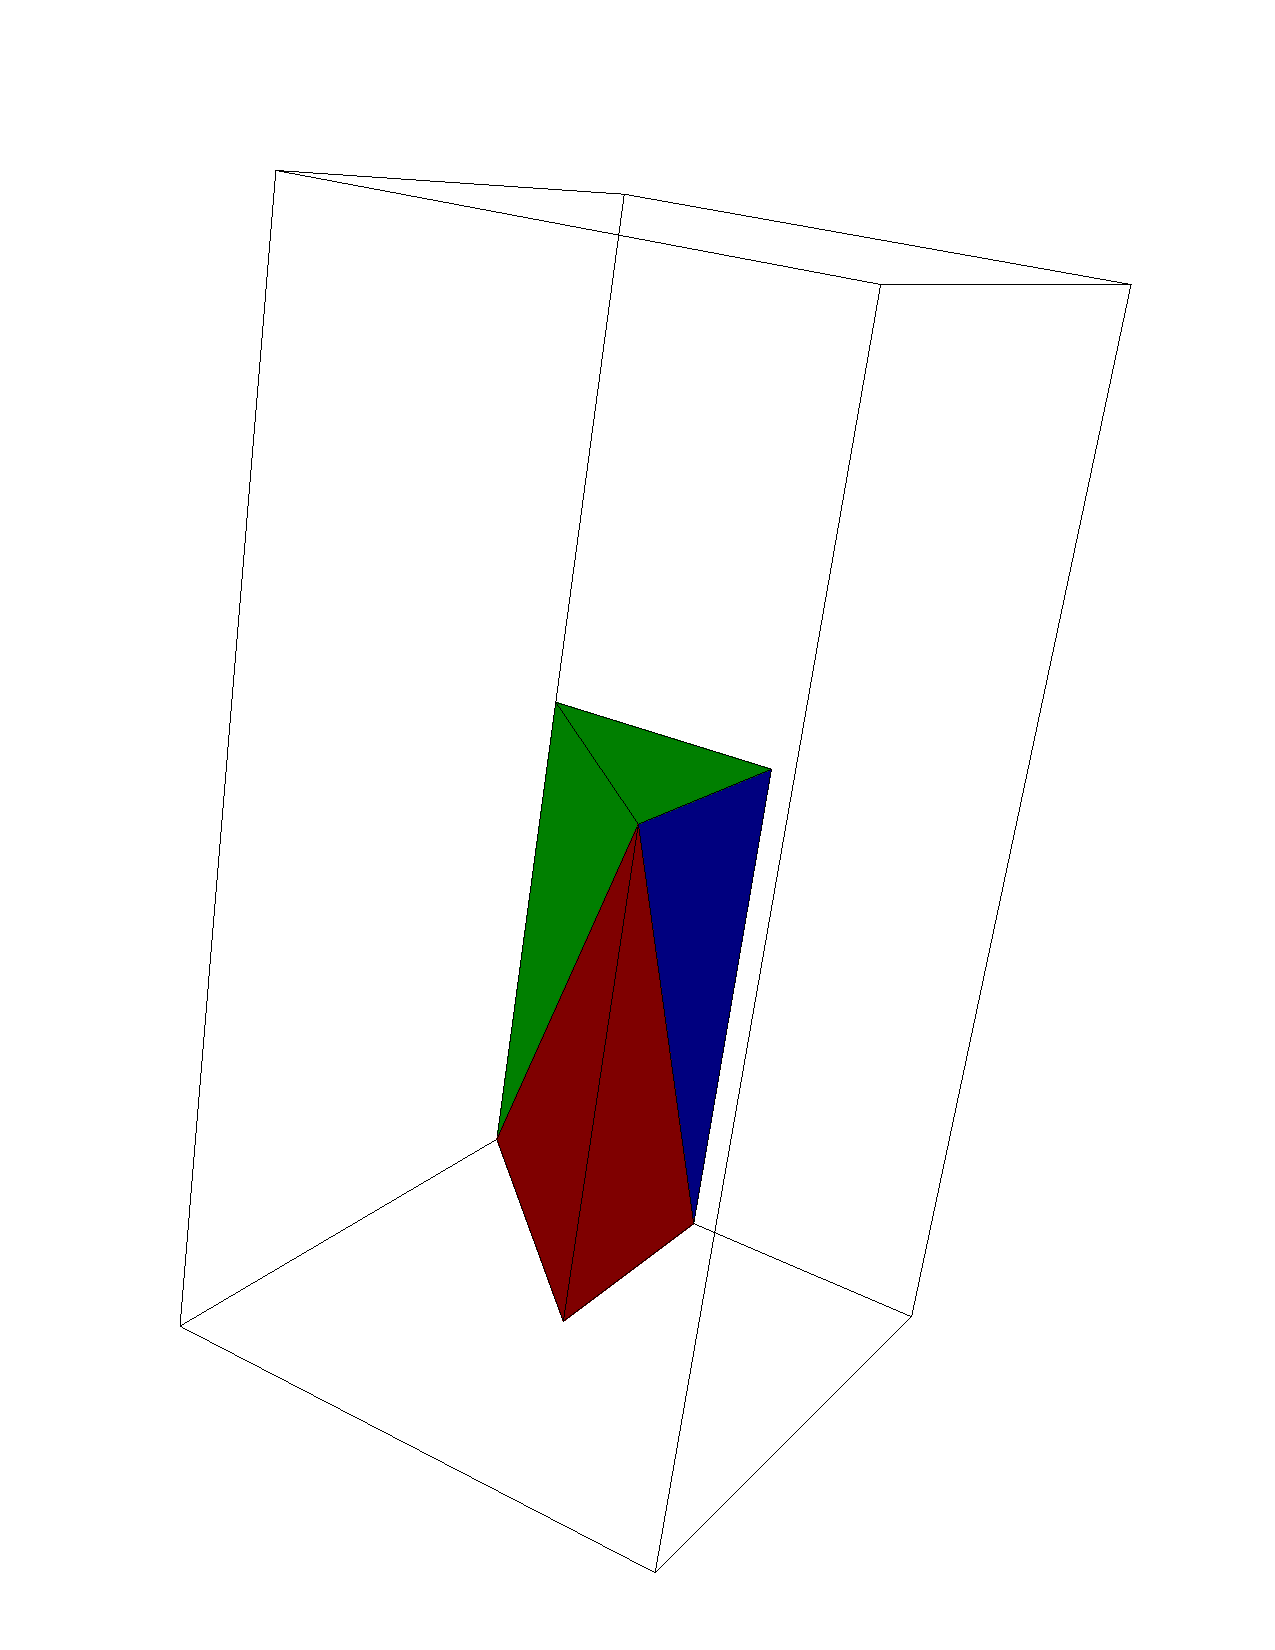
\includegraphics[width=0.4\textwidth]{hasab_bari.png}
\end{figure}

A szimplex pályákhoz tartozó multigráfot a \ref{abra:hasab_D-graf}. ábra
szemlélteti. Mivel minden szimplex pályára definiálva van minden szomszédsági
reláció, ezért az áttekinthetőség kedvéért azokat a relációkat nem ábrázoljuk,
melyek önmagára képezik le a pályát.
\begin{figure}
  \caption{\label{abra:hasab_D-graf} Hasábhoz tartozó multigráf}
  \center
  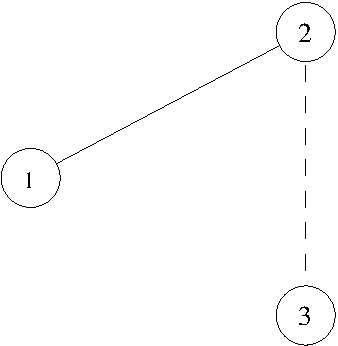
\includegraphics[width=0.2\textwidth]{hasab_D-graf.pdf}
\end{figure}

A mátrixfüggvények ($\mathcal{D}$ a szimplex pályák halmaza,
$D_i\in\mathcal{D}$):
\begin{equation*}
  \mathcal{R}(D_1)=
  \left(
  \begin{array}{cccc}
    1 & 1 & 2 & 1\\
    1 & 1 & 3 & 1\\
    2 & 3 & 1 & 2\\
    1 & 1 & 2 & 1
  \end{array}
  \right)
\end{equation*}
\begin{equation*}
  \mathcal{R}(D_2)=
  \left(
  \begin{array}{cccc}
    1 & 2 & 2 & 1\\
    2 & 1 & 3 & 2\\
    2 & 3 & 1 & 2\\
    1 & 2 & 2 & 1
  \end{array}
  \right)
\end{equation*}
\begin{equation*}
  \mathcal{R}(D_3)=
  \left(
  \begin{array}{cccc}
    1 & 2 & 1 & 1\\
    2 & 1 & 3 & 2\\
    1 & 3 & 1 & 1\\
    1 & 2 & 1 & 1
  \end{array}
  \right)
\end{equation*}

\begin{equation*}
  \forall D_i\in\mathcal{D}:\;
  \mathcal{M}(D_i)=
  \left(
  \begin{array}{cccc}
    1 & 4 & 2 & 2\\
    4 & 1 & 3 & 2\\
    2 & 3 & 1 & 4\\
    2 & 2 & 4 & 1
  \end{array}
  \right)
\end{equation*}


\subsection{D-szimbólum követelmények}
\label{D-sym-cond}
Az összes 3 dimenziós geometriában az összes lehetséges kövezés felsorolásához
szeretnénk a D-szimbólumokat felhasználni. A következő szükséges feltételeket
támasztjuk a D-szimbólumokkal szemben:
\begin{itemize}
  \item D-szimbólum absztrakt definíciója
  \item Megkötések $\mathcal{R}$ és $\mathcal{M}$ mátrixfüggvényekre (valódi
    vagy végtelen távoli szimplex csúcsok, jó orbifold feltételek)
\end{itemize}

\subsection{D-szimbólumok felsorolásához szükséges algoritmusok}
\subsubsection{D-diagramok felsorolása}
Rendezés bevezetése a D-diagramokra.

A használt algoritmus ismertetése. (Döntési fa modellel egyszerűen
szemléltethető.)

\subsubsection{A D-diagramokhoz tartozó mátrixfüggvények felsorolása}
Az $\mathcal{R}$ mátrixfüggvény és a paraméterek felírhatóak a D-diagram
alapján. A lehetséges $\mathcal{M}$ mátrixfüggvények illetve a hozzájuk tartozó
paraméterértékek pedig véges sokan vannak vagy végtelen láncokat alkotnak (lásd
\ref{D-sym-cond} fejezet: megkötések a mátrixfüggvényekre).

Rendezés bevezetése a teljes D-szimbólumra.

Algoritmus ismertetése.

\section{Továbblépések}
Ezek csak jegyzetek, gondolatmenetek.

\subsection{Adott D-szimbólumhoz tartozó fundamentális tartomány előállítása}
FIXME Megtehető konvex módon. Kérdés, hogy a ragasztás során végig konvex
marad-e a rendszer, vagy csak a legvégén. (Diplomamunkabeli D.109 esetén pl.
nem tud a rendszer végig konvex maradni.)

Mikor tud elromlani a konvexitás (ezeket a helyzeteket ki kell küszöbölni):
\begin{itemize}
  \item Pontosan akkor lesz az alakzat konkáv, ha van konkáv lapszöge
  \item Ha adott egy él, amit szimplexekkel körbe tudunk rakni ismétlés nélkül,
    a szimplexek "felénél többet", de nem az összeset ragasztjuk körbe az él
    körül. Ilyen éleket az irányitott (tükrözés mentes) 1 értékű paraméterek
    jelentenek.
  \item Ha egy élet csak ismétléssel tudunk körbe rakni, akkor nem tud konkáv
    lenni a hozzá tartozó lapszög.
\end{itemize}

További gondolatok:
\begin{itemize}
  \item Tükörképeket nem ragasztunk (ugyanazt a szimplexet 1-szer hasznaljuk fel
    a fundamentális tartomány ragasztásakor)
  \item Ha egy él körülrakásában van tükrözés, nem okoz gondot az él, mert lesz
    ismétlés a körberakásában.
  \item Ha nincs tükrözés, de legálabb 2-szer körbemegyünk (azaz a paraméter
    értéke legalább 2), szintén nem okoz gondot az él, mert lesz ismétlés a
    körberakásában.
  \item Ha 1 élet teljesen körbe rakunk szimplexekkel, akkor a fundamentális
    tartomány egy "belső élévé" változik, így nem alakít ki lapszöget.
  \item Azokat az eseteket kell tehát csak megvizsgálni, ahol több élet is körbe
    lehet rakni szimplexekkel ismétlés nélkül (vagyis irányított 1 paraméterű
    él-körből több is van.)
\end{itemize}

Az utolsó további gondolat folytatása és egy leendő algoritmus:
\begin{itemize}
  \item Vesszük az irányított 1 értékű paramétereket (él-körök), az általuk
    érintett szimplexek száma szerint csökkenő sorrendben
  \item Az első ilyenhez tartozó élet körbe ragasztjuk szimplexekkel.
  \item Megnézzük, hogy a maradék él-körök közül hány olyan van, aminek csak 1
    közös szimplexe van az eddig kiválasztott körök uniojával, vesszük a
    legnagyobb ilyet és kezdjük elölről az algoritmust (lásd \ref{ftrajz1}. és
    \ref{ftrajz13d} ábrák.)
    \begin{figure}
      \caption{\label{ftrajz1} Két irányított kör, 1 közös szimplexszel.}
      \center
      \includegraphics[width=0.4\textwidth]{fund-tart_rajz1.pdf}
    \end{figure}
    \begin{figure}
      \caption{\label{ftrajz13d} Két irányított kör, 1 közös szimplexszel
      fundamentális tartomány}
      \center
      \includegraphics[width=0.4\textwidth]{fund-tart_rajz13d.png}
    \end{figure}
  \item Megnézzük, hogy a maradék él-körök közül hány olyan van, aminek legalább
    2 közös szimplexe van az eddig kiválasztott körök uniojával. Vesszük azt,
    aminek a legtöbb szimplexe van még szabadon. \underline{Ezen} a ponton két eset
    lehetséges: 
    \begin{itemize}
      \item Ha a vizsgált él-kör minden foglalt szimplexe az él-kör szerint van
	ragasztva, akkor körberagaszthatjuk az él-kört.
      \item Ha van két szimplex ami az él-körrel nem kompatibilis módon van
	ragasztva, akkor kétoldalról elkezdjük összerakni a kört (lásd
	\ref{ftrajz2}. és \ref{ftrajz23d}. ábrák.) Fontos, hogy a maradék kört nem tudjuk körbe
	összeragasztani mert csak ekvivalens éleket jár körbe a két útvonal, de
	nem ugyanazt.
    \end{itemize}
    \begin{figure}
      \caption{\label{ftrajz2} Két irányított kör, 2 közös szimplexszel.}
      \center
      \includegraphics[width=0.4\textwidth]{fund-tart_rajz2.pdf}
    \end{figure}
    \begin{figure}
      \caption{\label{ftrajz23d} Két irányított kör, 2 közös szimplexszel
      fundamentális tartomány}
      \center
      \includegraphics[width=0.4\textwidth]{fund-tart_rajz23d.png}
    \end{figure}
  \item A maradék szimplexek között megnézzük, hogy van-e még él-kör, ha igen,
    a maradékra is végrehajtjuk a fenti algoritmust
  \item Mostanra kaptunk néhány (esetleg 1 elemű) komponenst, melyeket szabadon
    összeragaszthatunk egy-egy operáció mentén, mert a "veszélyes" éleket már
    hatástalanítottuk. \underline{Felmerül} a kérdés, hogy miért nem fordulhat elő olyan
    eset, hogy egy "veszélyes" él-kört kontrollálatlanul ragasztunk körbe.
\end{itemize}

\subsection{Generátorok és relációk}
Először a fundamentális tartományt kell felépíteni.

\subsection{Schönfliess-Bieberbach tétel általánosítása}
Sch-B tétel kimondása.

A Schönflies-Bieberbach tételt általánosíthatjuk tetszőleges geometriára
úgy, hogy rácsok helyett fixpont mentes egybevágóságokat vizsgálunk.

Írunk egy módszert, ami egy adott D-szimbólumhoz előállít egy fixpont mentes
egybevágóságcsoportot leíró "felfújt" D-szimbólumot.

Az algoritmus:
\begin{itemize}
  \item Javított első lépés: Megnézzük az ekvivalens tükrözéseket. Mit is jelent
    ez: A súlyzó alakú rendszereket ki kell javítani vele (lásd \ref{schrajz2}.
    ábra, a D-szimbólumokhoz tartozó szimmetria-töréses kockakövezés
    fundamentális tartományát lásd \ref{schrajz23d}. ábra) Hogyan lehet továbblépni?
    \begin{figure}
      \caption{\label{schrajz2} Tükrözések felbontása 2.}
      \center
      \includegraphics[width=0.3\textwidth]{sch-b-alt_rajz2.pdf}
    \end{figure}
    \begin{figure}
      \caption{\label{schrajz23d} Tükrözések felbontása 2-höz tartozó
      fundamentális tartományok}
      \center
      \includegraphics[width=0.3\textwidth]{sch-b-alt_rajz23d1.png}
      \includegraphics[width=0.3\textwidth]{sch-b-alt_rajz23d2.png}
    \end{figure}
  \item Új verzió: Az összes élet vizsgáljuk:
    \begin{enumerate}
      \item \underline{Ez az elgondolás hibás}, erre részben a fundamentális tartomány
	döbbentett rá: Sorra vesszük a nem iranyítottan (tükrözés segítségével) körberakott
	éleket. Minden ilyet megszüntetünk úgy, hogy a körberakáshoz tartozó
	paraméter duplájaszor lemásoljuk a teljes D-szimbólumot, és a
	tükrözött szimplexeket és másolataikat kapcsoljuk össze a tükrözés
	operátorával (lásd \ref{schrajz3}. ábra fundamentális tartományok
	\ref{schrajz33d}. ábrán.) Ez a módszer szabadon el tudja rontani az
	operáció-párok rendjét, amit nem is tudunk egyszerűen kiküszöbölni.
	\begin{figure}
	  \caption{\label{schrajz3} Irányítatlan kör felbontása}
	  \center
	  \includegraphics[width=0.75\textwidth]{sch-b-alt_rajz3.pdf}
	\end{figure}
	\begin{figure}
	  \caption{\label{schrajz33d} Irányítatlan kör felbontás fundamentális
	  tartománya, ami egy belső szimmetria nélküli oktaéder}
	  \center
	  \includegraphics[width=0.75\textwidth]{sch-b-alt_rajz33d.png}
	\end{figure}
      \item Sorra vesszük az irányítottan (tükrözés nélkül) körberakott éleket.
	Minden ilyet megszüntetünk úgy, hogy először szétvágjuk a kört egy
	tetszőleges helyen, majd a körberakáshoz tartozó paraméterszer
	lemásoljuk a teljes szétvágott D-szimbólumot, és a vágáshoz betoldjuk
	(lásd \ref{schrajz4}. ábra, hozzá tartozó fundamentális tartomány:
	\ref{schrajz43d}. ábra) Itt nem látom, hogy a módszer elrontaná
	valamelyik operáció-párok rendjét.
	\begin{figure}
	  \caption{\label{schrajz4} Irányított kör felbontása}
	  \center
	  \includegraphics[width=0.75\textwidth]{sch-b-alt_rajz4.pdf}
	\end{figure}
	\begin{figure}
	  \caption{\label{schrajz43d} Irányított kör felbontása fundamentális
	  tartomány}
	  \center
	  \includegraphics[width=0.75\textwidth]{sch-b-alt_rajz43d.png}
	\end{figure}
    \end{enumerate}
  \item \underline{Legújabb verzió}: Az irányítottan körberakott éleket az előző verzió
    szerint kezeljük. A tükrözést is tartalmazó körberakásokhoz használható
    lehet a fundamentális tartomány felírása (a határoló lapok egymásba-simulása
    értékes információ.) Vagy a következő kicsi lépések, amikkel csak kezelhető
    mennyiségű paraméter változik 1-1 lépésben. Mindig egy nem szomszédos
    operáció-párhoz tartozó súlyzót (vagy dupla hurkot) bontunk szét. Ezzel
    megtöbbszörözzük (vagy megpáros-szorozzuk) a D-szimbólumot. Ezek a
    lépések választhatók úgy, hogy a megfelelő paramétert elérjük, ekkor
    visszatérünk a kiindulási ponthoz. (Ez akkor jó, ha 2 oldala van a
    szimbólumnak (lásd \ref{schrajz5}. ábra.) Minden tükrözést tartalmazó
    él-körnek a két szélén (a hurkoknál) ki kell alakuljon legalább egy súlyzó
    vagy dupla-hurok; ezt kéne kihasználni.
    \begin{figure}
      \caption{\label{schrajz5} Irányított kör felbontása}
      \center
      \includegraphics[width=0.75\textwidth]{sch-b-alt_rajz5.pdf}
    \end{figure}
\end{itemize}


  \end{document}
